% ICL modality-gating paper — ACL/EMNLP Findings (ARR) target.
% Self-contained preamble so it compiles standalone; to use the official ACL style,
% replace the preamble with \documentclass[11pt]{article}\usepackage[review]{acl} etc.
\documentclass[11pt]{article}
\usepackage[margin=1in]{geometry}
\usepackage{times}
\usepackage{graphicx}
\usepackage{booktabs}
\usepackage{amsmath}
\usepackage{multirow}
\usepackage{xcolor}
\usepackage[round]{natbib}
\usepackage[hidelinks]{hyperref}
\usepackage{authblk}
\title{\bf When Does Few-Shot Help? Input-Format Novelty Gates\\
In-Context Learning via Task Recognition}
\author[ ]{Anonymous (ARR submission)}
\affil[ ]{ }
\date{}

\begin{document}
\maketitle

\begin{abstract}
In-context learning (ICL) is widely treated as a general-purpose lever for adapting
large language models (LLMs). We show that its benefit is sharply \emph{conditional}:
few-shot demonstrations help an order of magnitude more when the input is presented
in a \emph{format the model is unfamiliar with}, and barely at all otherwise.
Using a controlled testbed---the same underlying task rendered in a familiar versus an
alien surface format---we find across six instruction-tuned LLMs (3 families, 3 scales)
that ICL gain on a novel numeric format (Korean facial Action-Unit intensities as text)
reaches $+6.7$ to $+16.4$ points, while on familiar English dialog it is $\le 5$ points.
A label-ablation (gold vs.\ random demonstration labels) shows the gain is
$\sim$75\% \emph{task recognition}, not task learning: demonstrations help the model
\emph{recognize} a latent task that the unfamiliar format hides, rather than teach a new
mapping. We further show (i) the effect is \emph{not} explained by input perplexity
(the novel format is in fact the \emph{lowest}-perplexity input; Spearman
$\rho=-0.72$) but tracks tokenizer \emph{fertility}
(Pearson $r=0.70$, $p{=}0.001$, $n{=}18$), a corpus-free format-novelty measure; (ii) it replicates
in a second, non-emotion domain (sentiment under a leetspeak encoding, where zero-shot
collapses $92\!\to\!58$\% and ICL partially restores it); and (iii) it requires
\emph{both} a latently-known task \emph{and} a novel format---a novel format alone, on a
task the model cannot do (serialized clinical tables), yields no ICL gain. One model
family (Mistral) is a consistent exception across both domains, which we tie to
pretraining-corpus composition. Our results refine \emph{when} practitioners should
expect ICL to pay off and supply a cheap predictor for it.
\end{abstract}

\section{Introduction}
Practitioners reach for in-context learning (ICL) as a default adaptation tool, often
assuming a few demonstrations reliably improve an LLM on a new task. Yet the size of the
ICL benefit varies enormously and unpredictably across tasks. We ask a sharper question:
\emph{holding the underlying task fixed, what property of the input makes few-shot
demonstrations help?}

We isolate \textbf{input-format novelty} as a causal factor. Our central testbed
presents a task the LLM already has latent competence for, in two surface formats: a
\emph{familiar} natural-language rendering and a \emph{novel}, alien encoding (e.g.\
numeric feature codes). The novel format collapses zero-shot accuracy; the question is
whether and why demonstrations recover it.

\begin{figure*}[t]\centering
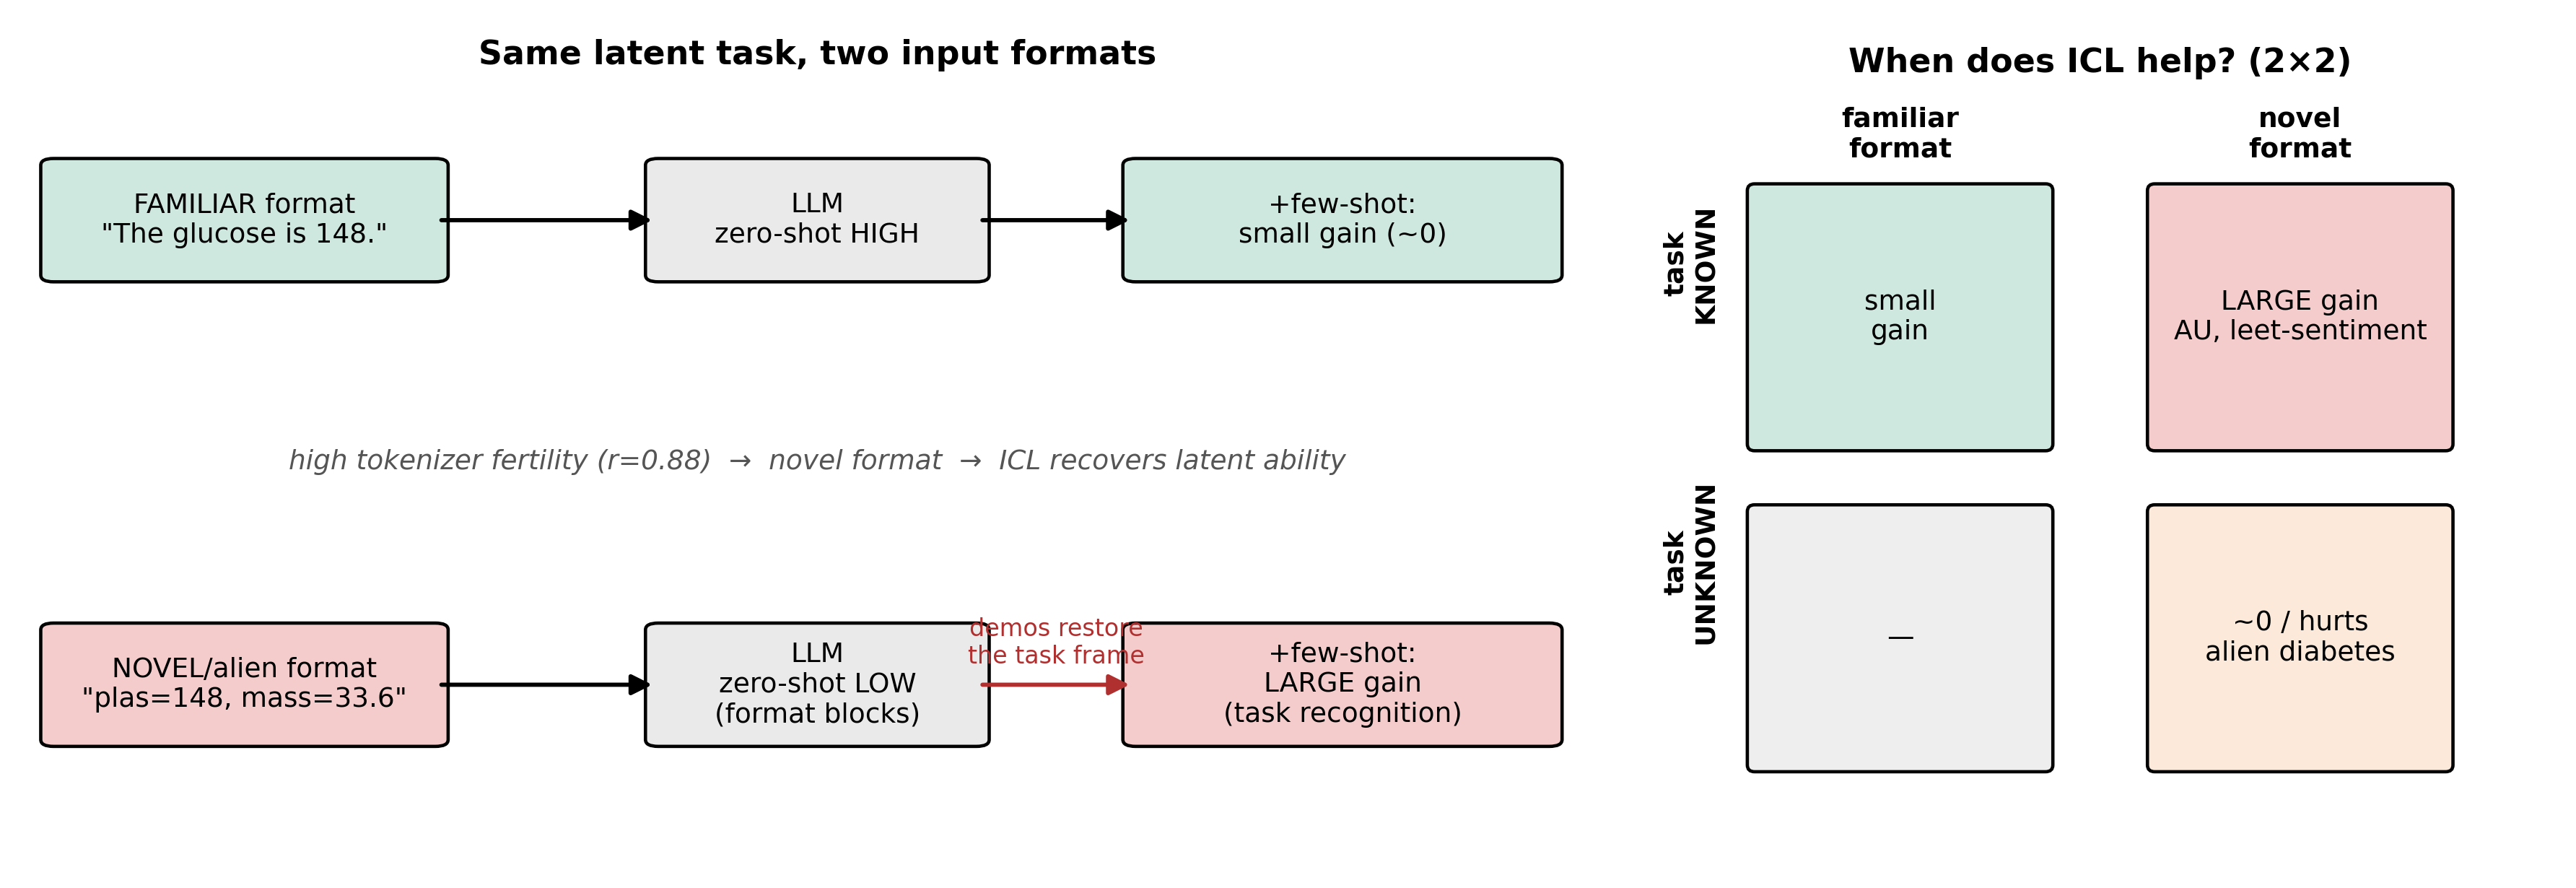
\includegraphics[width=0.95\linewidth]{figures/fig1_concept.png}
\caption{\textbf{Format-novelty gating.} (left) For the \emph{same} latently-known task,
a familiar input format keeps zero-shot high and few-shot adds little; an unfamiliar
format collapses zero-shot, and few-shot demonstrations restore performance by
re-establishing the task frame (\emph{task recognition}). (right) The gain appears only
when the task is latently known \emph{and} the format is novel.}\label{fig:concept}
\end{figure*}

Our contributions are:
\begin{enumerate}\itemsep0pt
\item A robust \textbf{format-novelty gating} effect: ICL gain is much larger on a novel
input format than a familiar one, replicated across 5/6 LLMs and three model families
(\S\ref{sec:gating}).
\item A \textbf{mechanism}: via a gold-vs-random label ablation, the gain is
$\sim$75\% \emph{task recognition} (random-label-robust), not task learning---demonstrations
help the model recognize a latent task that the format hides (\S\ref{sec:mech}).
\item A cheap \textbf{format-novelty signal}: tokenizer \emph{fertility} tracks ICL gain
across formats ($r=0.70$, $n{=}18$) where input perplexity \emph{fails} ($\rho=-0.72$) (\S\ref{sec:pred}).
\item \textbf{Cross-domain generalization and boundary conditions}: the effect reappears
in sentiment under a leetspeak encoding, and vanishes when the task itself is not
latently known (clinical tables), giving a clean
$2\times2$ (\S\ref{sec:second},\ref{sec:boundary}).
\item Negative controls ruling out perplexity, headroom, and representation compaction,
plus an analysis of the one exception family (\S\ref{sec:controls}).
\end{enumerate}

\section{Related Work}
\textbf{When does ICL work.} \citet{min2022rethinking} show that for familiar tasks,
ground-truth demonstration labels barely matter---demonstrations mainly convey the label
space and format. \citet{pan2023tr} formalize this as \emph{task recognition} (TR,
random-label-robust) vs.\ \emph{task learning} (TL). We extend this distinction to
\emph{novel input formats}: we show \emph{when the format itself}, not the task, triggers
a large TR-dominant gain, and we supply a predictor and a falsifying negative that prior
TR/TL work (run only on familiar English text) does not.
\textbf{Representation of the input.} \citet{fu2024isobench} document that isomorphic
representations of the same task yield very different LLM accuracy, and tabular-LLM work
\cite{hegselmann2023tabllm} shows serialization choice swings few-shot accuracy; neither
runs the label ablation that isolates the mechanism. Cipher-reasoning
results indicate that \emph{too} alien an encoding is not recoverable by demonstrations,
bounding our ``recoverable-novelty'' window.
\textbf{Pretraining dependence.} ICL emergence depends on pretraining-corpus composition
\cite{shin2022corpora} and on whether a task family lies in the pretraining mixture
\cite{yadlowsky2023mixtures}; we use this to explain our one exception family.
\textbf{Format-familiarity proxies.} \citet{razeghi2022impact} tie few-shot accuracy to
pretraining term frequency; we use \emph{tokenizer fertility} as a corpus-free,
format-level analogue.

\section{Experimental Setup}
\textbf{Task and formats.} Each cell is (model $\times$ input format). The primary novel
format is Korean facial Action-Unit (AU) intensities serialized as text
(e.g.\ ``\texttt{plas=148, mass=33.6, \dots}'' style), a 4-class emotion task; AU labels
derive from a large Korean corpus validated by a 298-annotator consensus study. Familiar
inputs are English dialog emotion (IEMOCAP, MELD). For each cell we measure zero-shot,
gold-label ICL ($k{=}4$), and random-label ICL accuracy ($N{=}400$, balanced, 5--7 seeds).
\textbf{Models.} Qwen2.5-\{3B,7B,14B\}, Yi-1.5-6B, Falcon3-7B, Mistral-7B-Instruct,
all 4-bit, greedy decoding.
\textbf{Metrics.} ICL gain $=$ gold$-$zero; $\mathrm{TR}=$ random$-$zero;
$\mathrm{TL}=$ gold$-$random; fertility $=$ tokens-per-word of the format schema.
We avoid prompt-scaffolding confounds by using a minimal prompt with no task-specific
hints (\S\ref{sec:controls}).

\section{Results}
\subsection{Format-novelty gates ICL}\label{sec:gating}
Table~\ref{tab:gating} and Fig.~\ref{fig:gating} show ICL gain per cell. On the novel AU
format, gain is large for five of six models---Qwen-3B/7B/14B $+6.7/+16.4/+14.5$,
Yi-6B $+10.5$, Falcon-7B $+14.7$---versus $\le5$ on familiar dialog. Mistral is the lone
exception ($+1.2$).

\begin{table}[t]\centering\small
\begin{tabular}{lccc}
\toprule
Model & AU (novel) & IEMOCAP & MELD\\
\midrule
Qwen2.5-3B  & $+6.7$  & $+1.8$ & $-2.1$\\
Qwen2.5-7B  & $+16.4$ & $+1.6$ & $-0.7$\\
Qwen2.5-14B & $+14.5$ & $+4.9$ & $+3.8$\\
Yi-1.5-6B   & $+10.5$ & $+5.9$ & $+2.0$\\
Falcon3-7B  & $+14.7$ & $+3.7$ & $+1.5$\\
Mistral-7B  & $+1.2$  & $+2.4$ & $-1.8$\\
\bottomrule
\end{tabular}
\caption{ICL gain (pp, gold$-$zero) per model and input format. Novel format (AU)
dominates familiar dialog for 5/6 models.}\label{tab:gating}
\end{table}

\begin{figure}[t]\centering
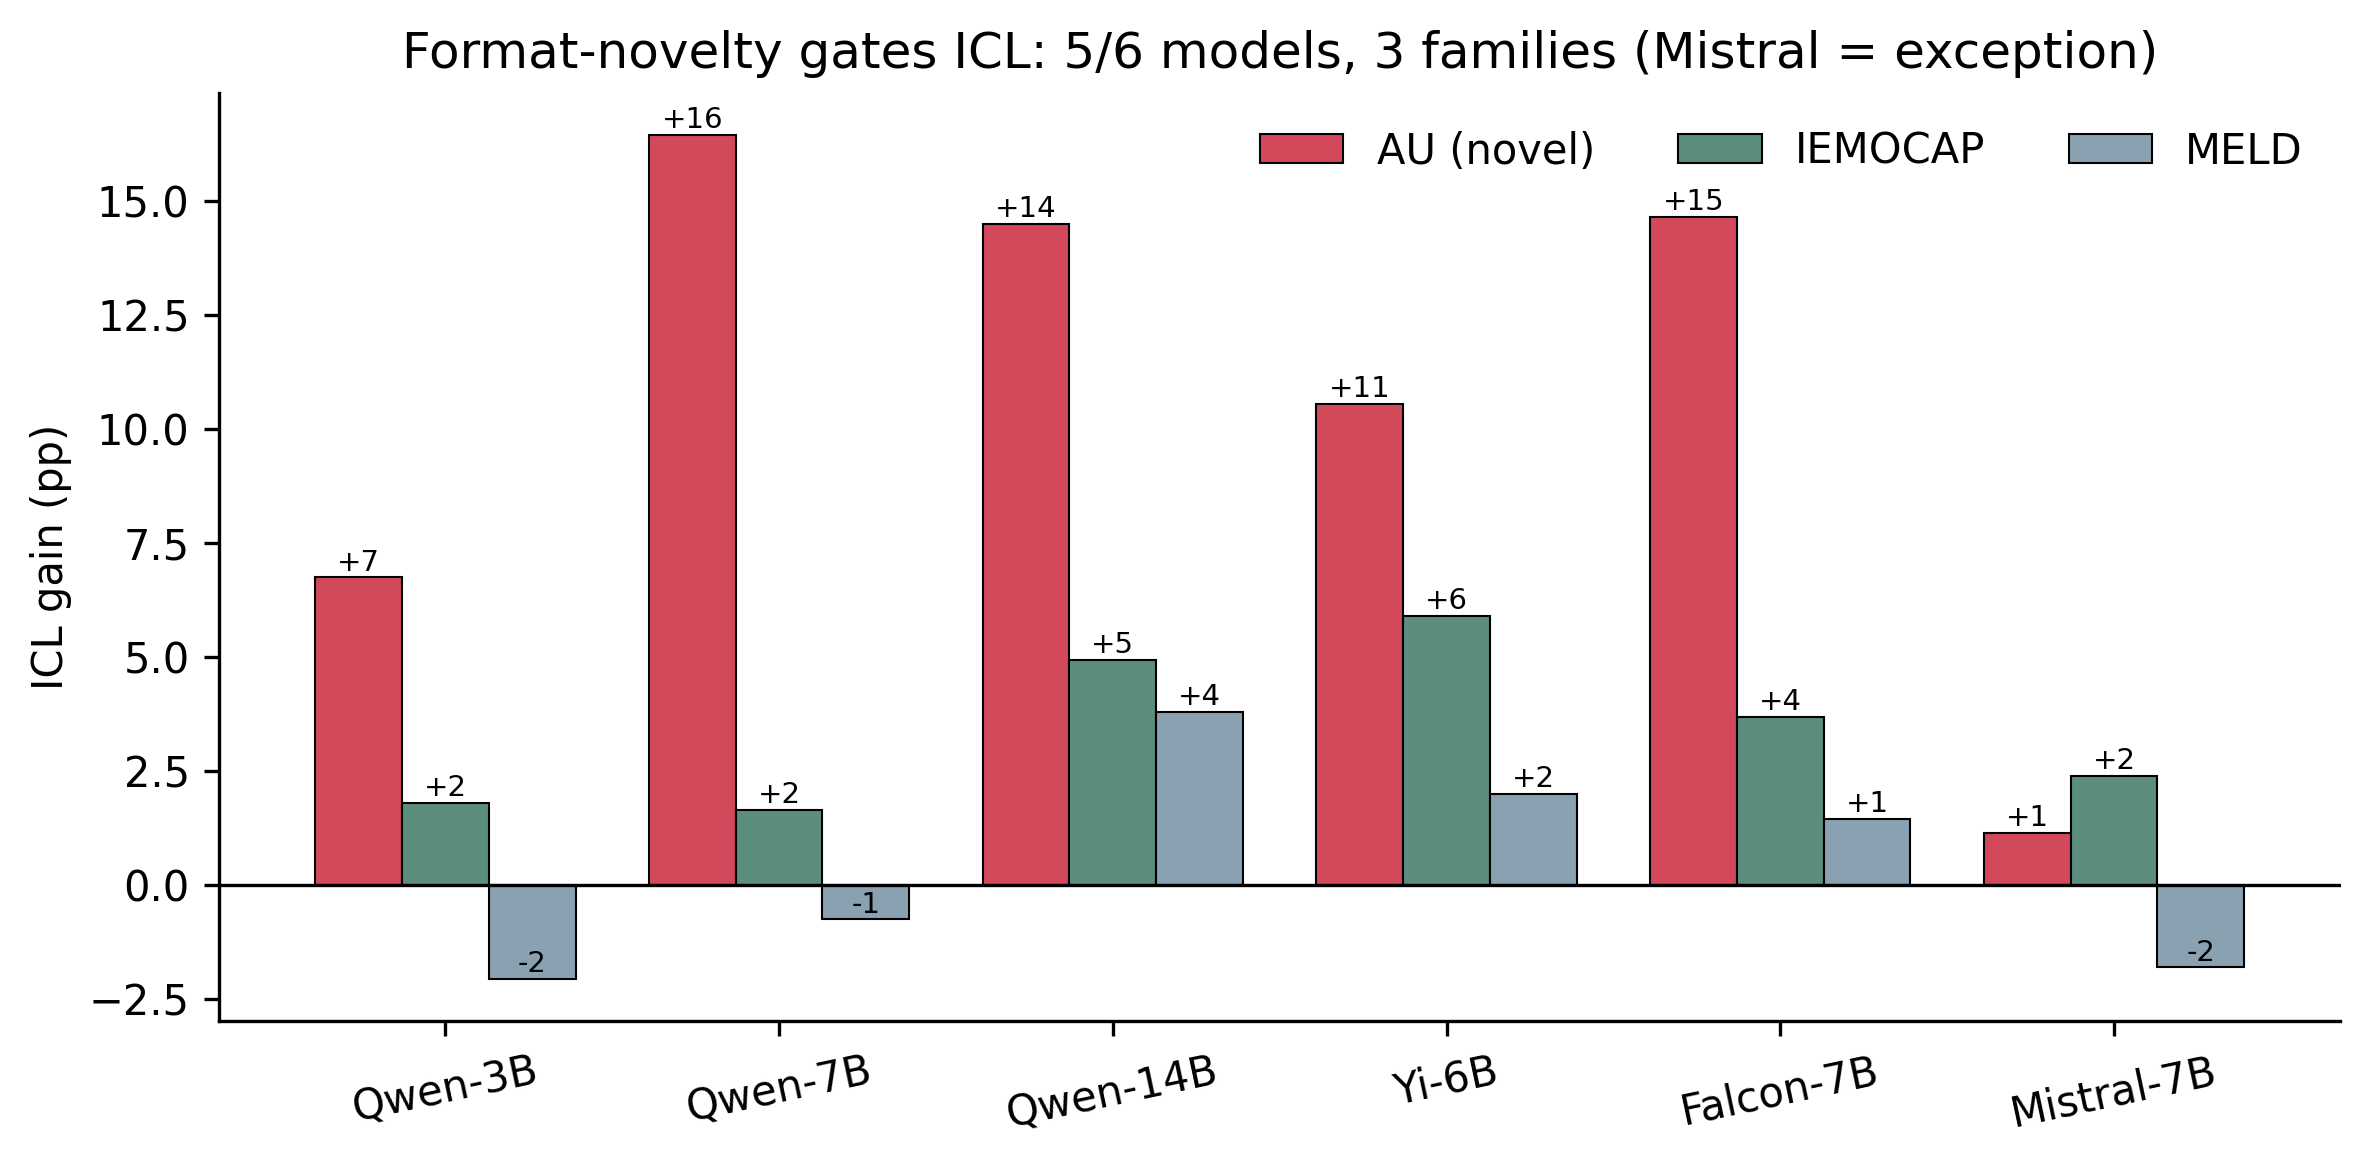
\includegraphics[width=\linewidth]{figures/figA_gating_6model.png}
\caption{Format-novelty gates ICL across six models / three families.}\label{fig:gating}
\end{figure}

\subsection{The gain is task recognition}\label{sec:mech}
Replacing gold demonstration labels with random labels barely reduces the AU gain
(Fig.~\ref{fig:mech}): the gain decomposes into $\sim$75\% TR and little TL
(Qwen-7B 89\%, Qwen-14B 80\%, Yi-6B 70\%, Falcon-7B 72\% TR). Because random labels
preserve the gain, demonstrations are not teaching the AU$\to$emotion mapping; they help
the model \emph{recognize} a task it already latently knows but cannot access from the
unfamiliar format cold. On familiar dialog, TR is near zero---no recognition is needed.

\begin{figure}[t]\centering
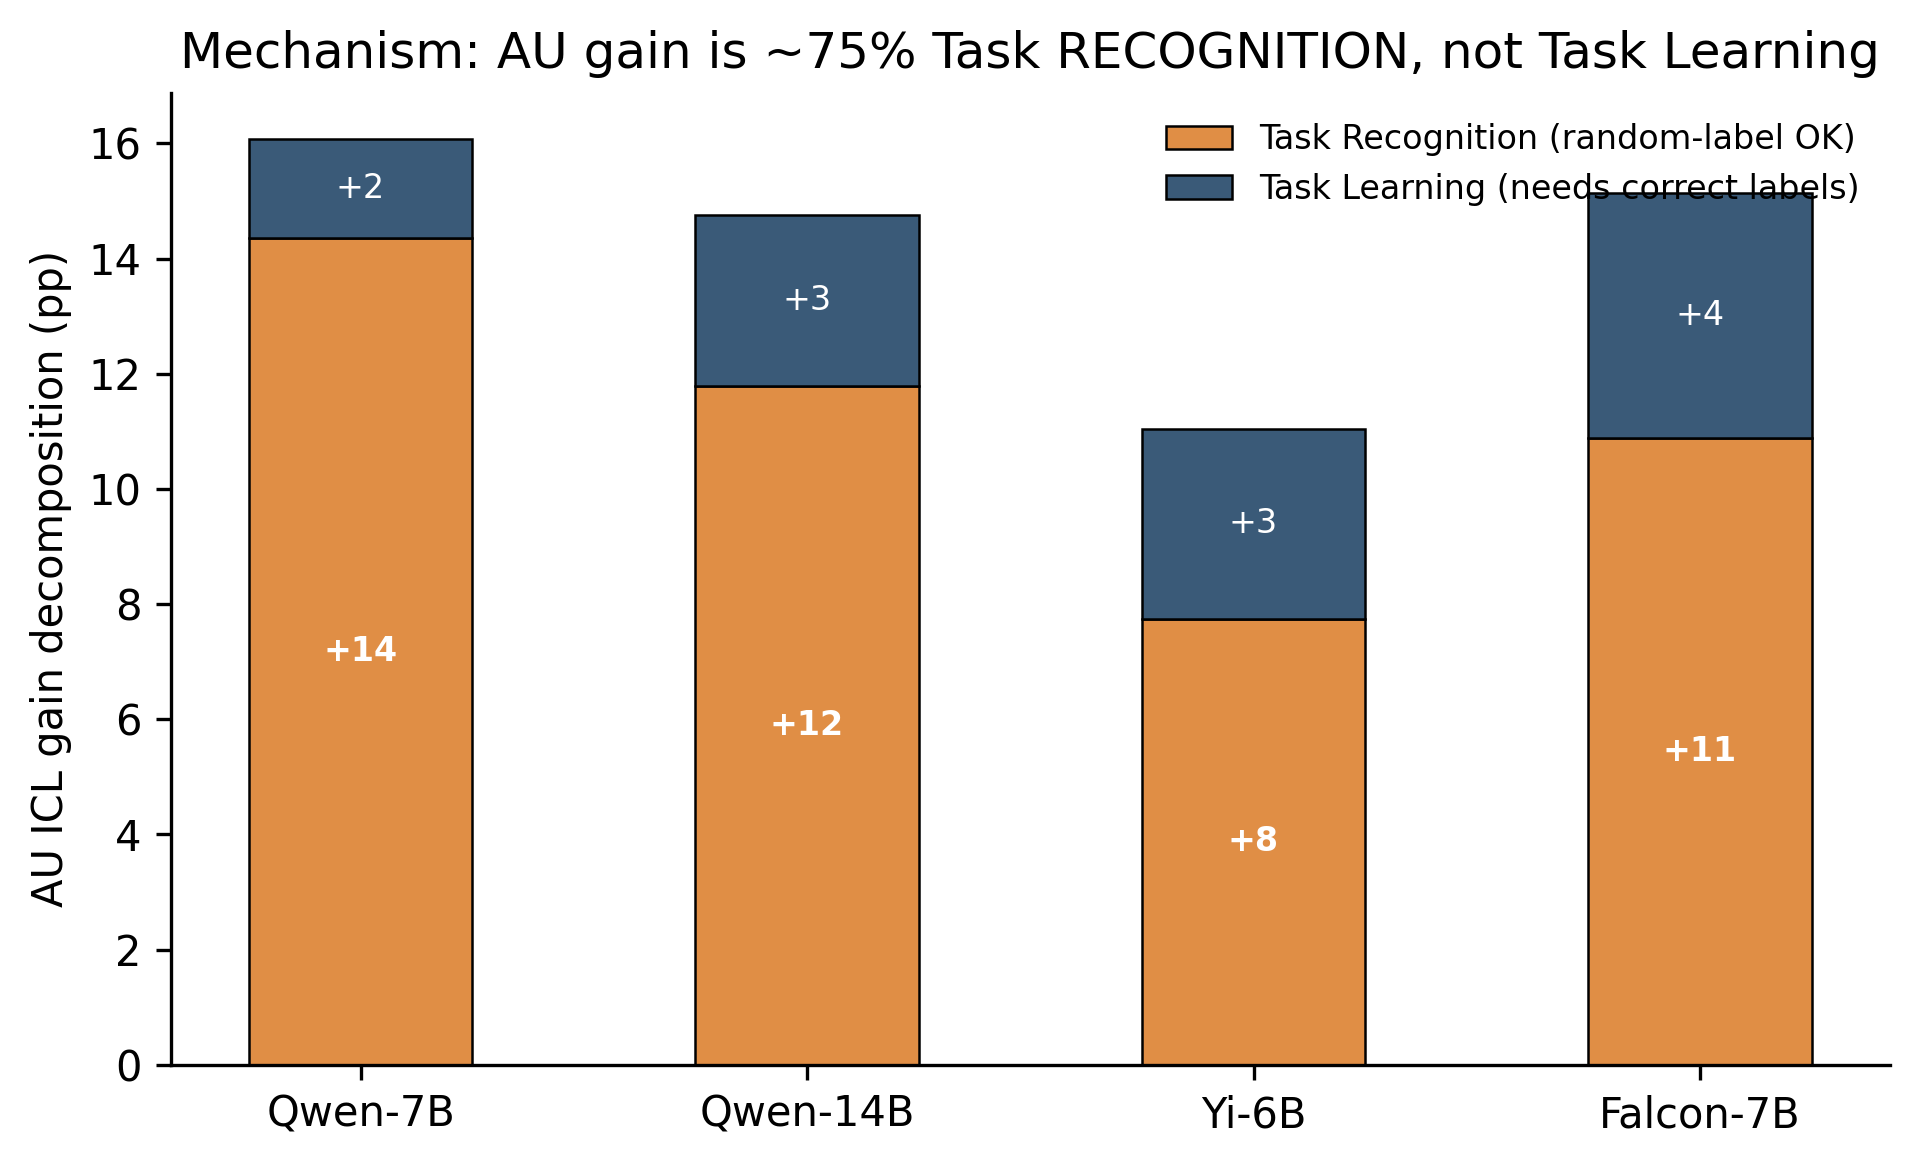
\includegraphics[width=0.9\linewidth]{figures/figC_mechanism_TRTL.png}
\caption{AU ICL gain is $\sim$75\% task recognition (random-label-robust), not task
learning.}\label{fig:mech}
\end{figure}

\subsection{Fertility predicts the gain; perplexity does not}\label{sec:pred}
A natural hypothesis is that ICL helps on ``surprising'' inputs. It does \emph{not}: the
AU format is the \emph{lowest}-perplexity input, and per-token NLL correlates
\emph{negatively} with gain (Spearman $\rho=-0.72$). Instead, tokenizer \emph{fertility}
(tokens-per-word of the schema) correlates \emph{positively} with gain across all six models
($r=0.70$, $p{=}0.001$, $n{=}18$, bootstrap 95\% CI $[0.38,0.90]$; Fig.~\ref{fig:perp}): the
novel format fragments into many tokens because its surface form is rare, and that
format-level novelty---not token surprise---is what ICL compensates for. The signal is
\emph{between-format}: fertility cleanly separates the novel AU schema (mean $3.2$) from
familiar dialog ($1.7$), but does not rank-order gain \emph{within} the familiar formats
(within-family Spearman $\rho{=}{-}0.09$, n.s.). We therefore read fertility as an a-priori
indicator of \emph{which} formats are novel enough to benefit, not a graded dose--response.

\begin{figure}[t]\centering
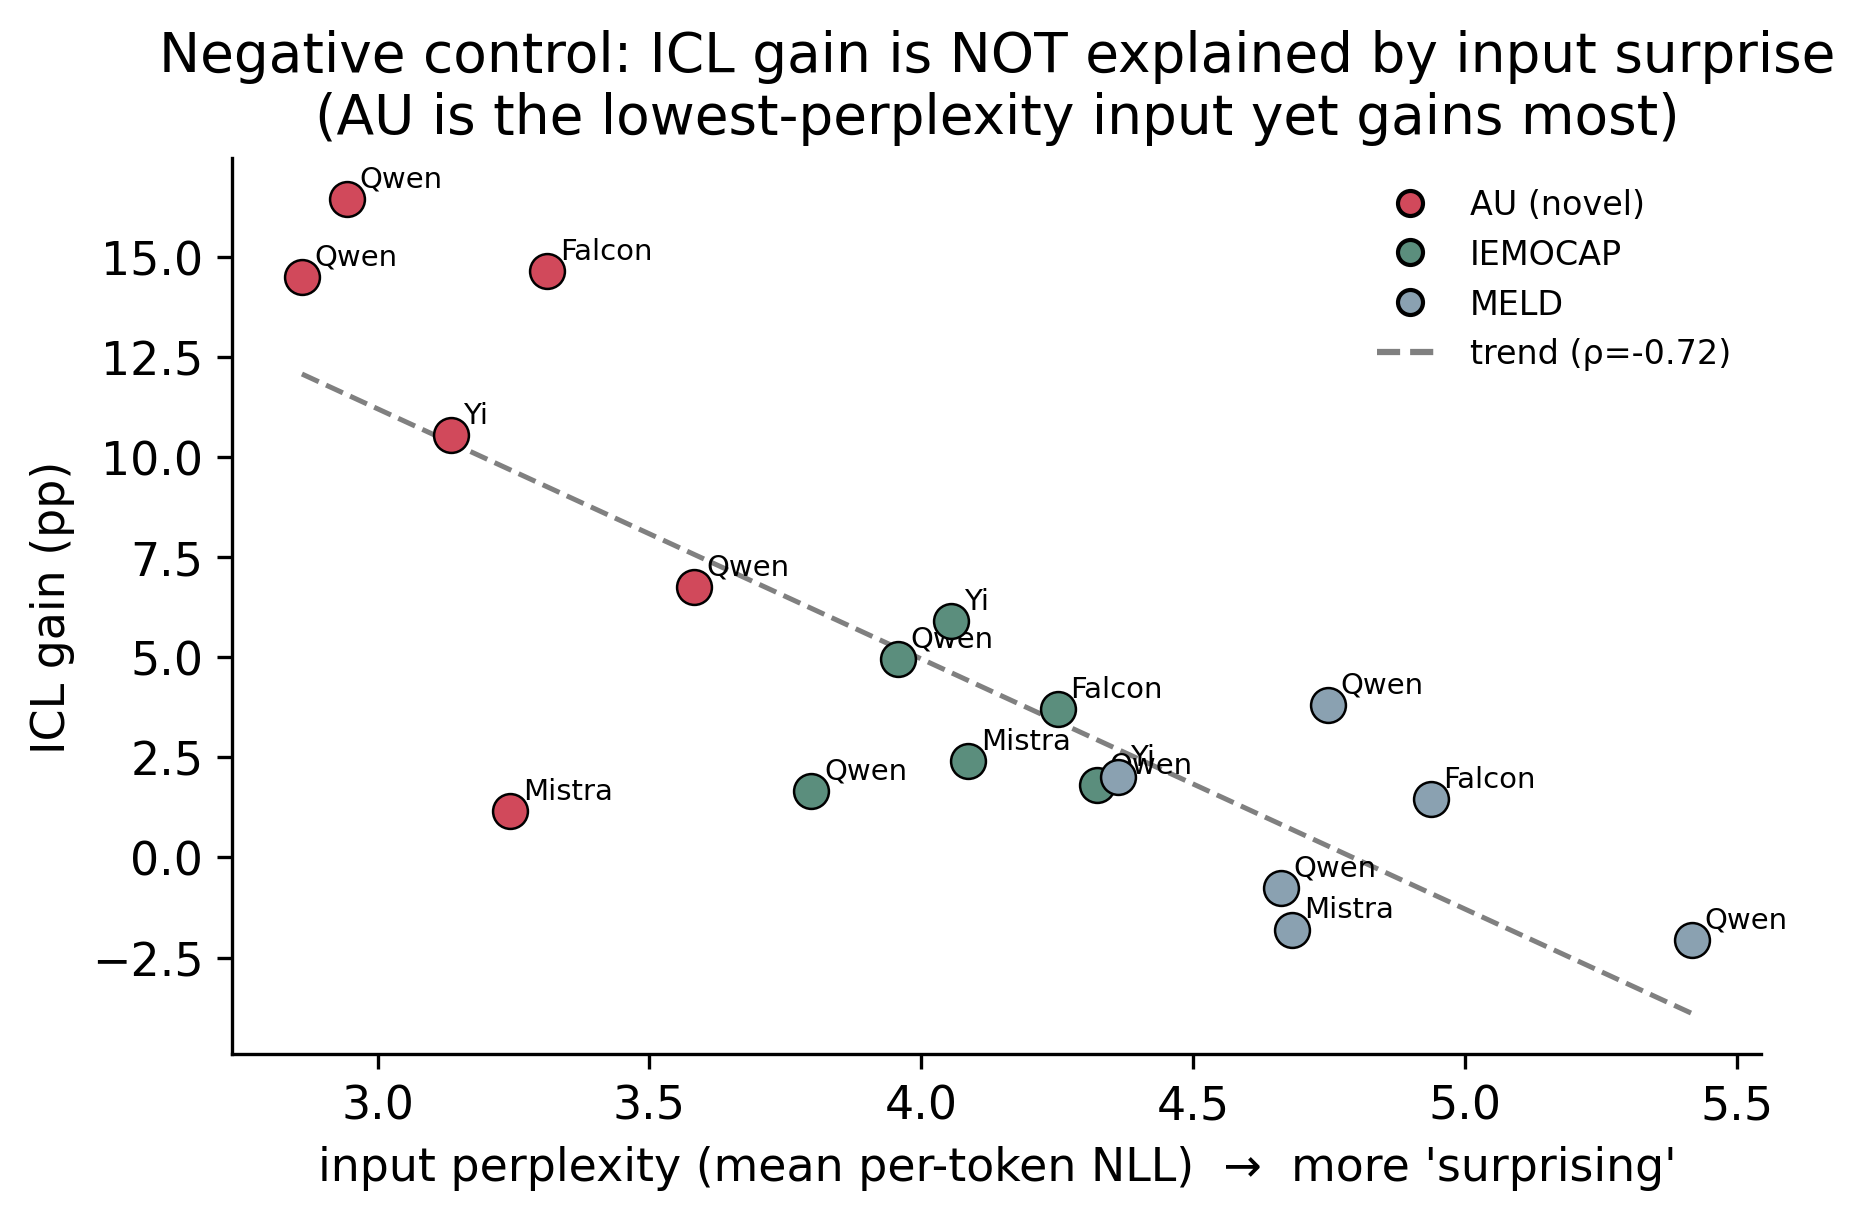
\includegraphics[width=0.9\linewidth]{figures/figB_perplexity_control.png}
\caption{Negative control: ICL gain is \emph{not} explained by input perplexity (the
novel AU format is lowest-perplexity yet gains most).}\label{fig:perp}
\end{figure}

\subsection{A second, non-emotion domain}\label{sec:second}
We replicate the effect on sentiment (SST-2), a task LLMs do well ($>$90\% zero-shot),
by re-encoding reviews in \emph{leetspeak} (``\texttt{th15 m0v13 15 4m4z1ng}''), holding
content fixed. The alien encoding collapses Qwen-7B zero-shot $92.3\!\to\!57.8$\%;
ICL then gives $+5.7$ vs.\ $+2.7$ in the plain format ($\Delta{=}{+}3.0$). The effect is
TR-driven and positive for 3/4 models (Falcon-7B $\Delta{=}{+}8.2$), with Mistral again
the exception ($\Delta{=}{-}4.7$). Fig.~\ref{fig:cross} shows the format-novelty effect
across both domains.

\begin{figure}[t]\centering
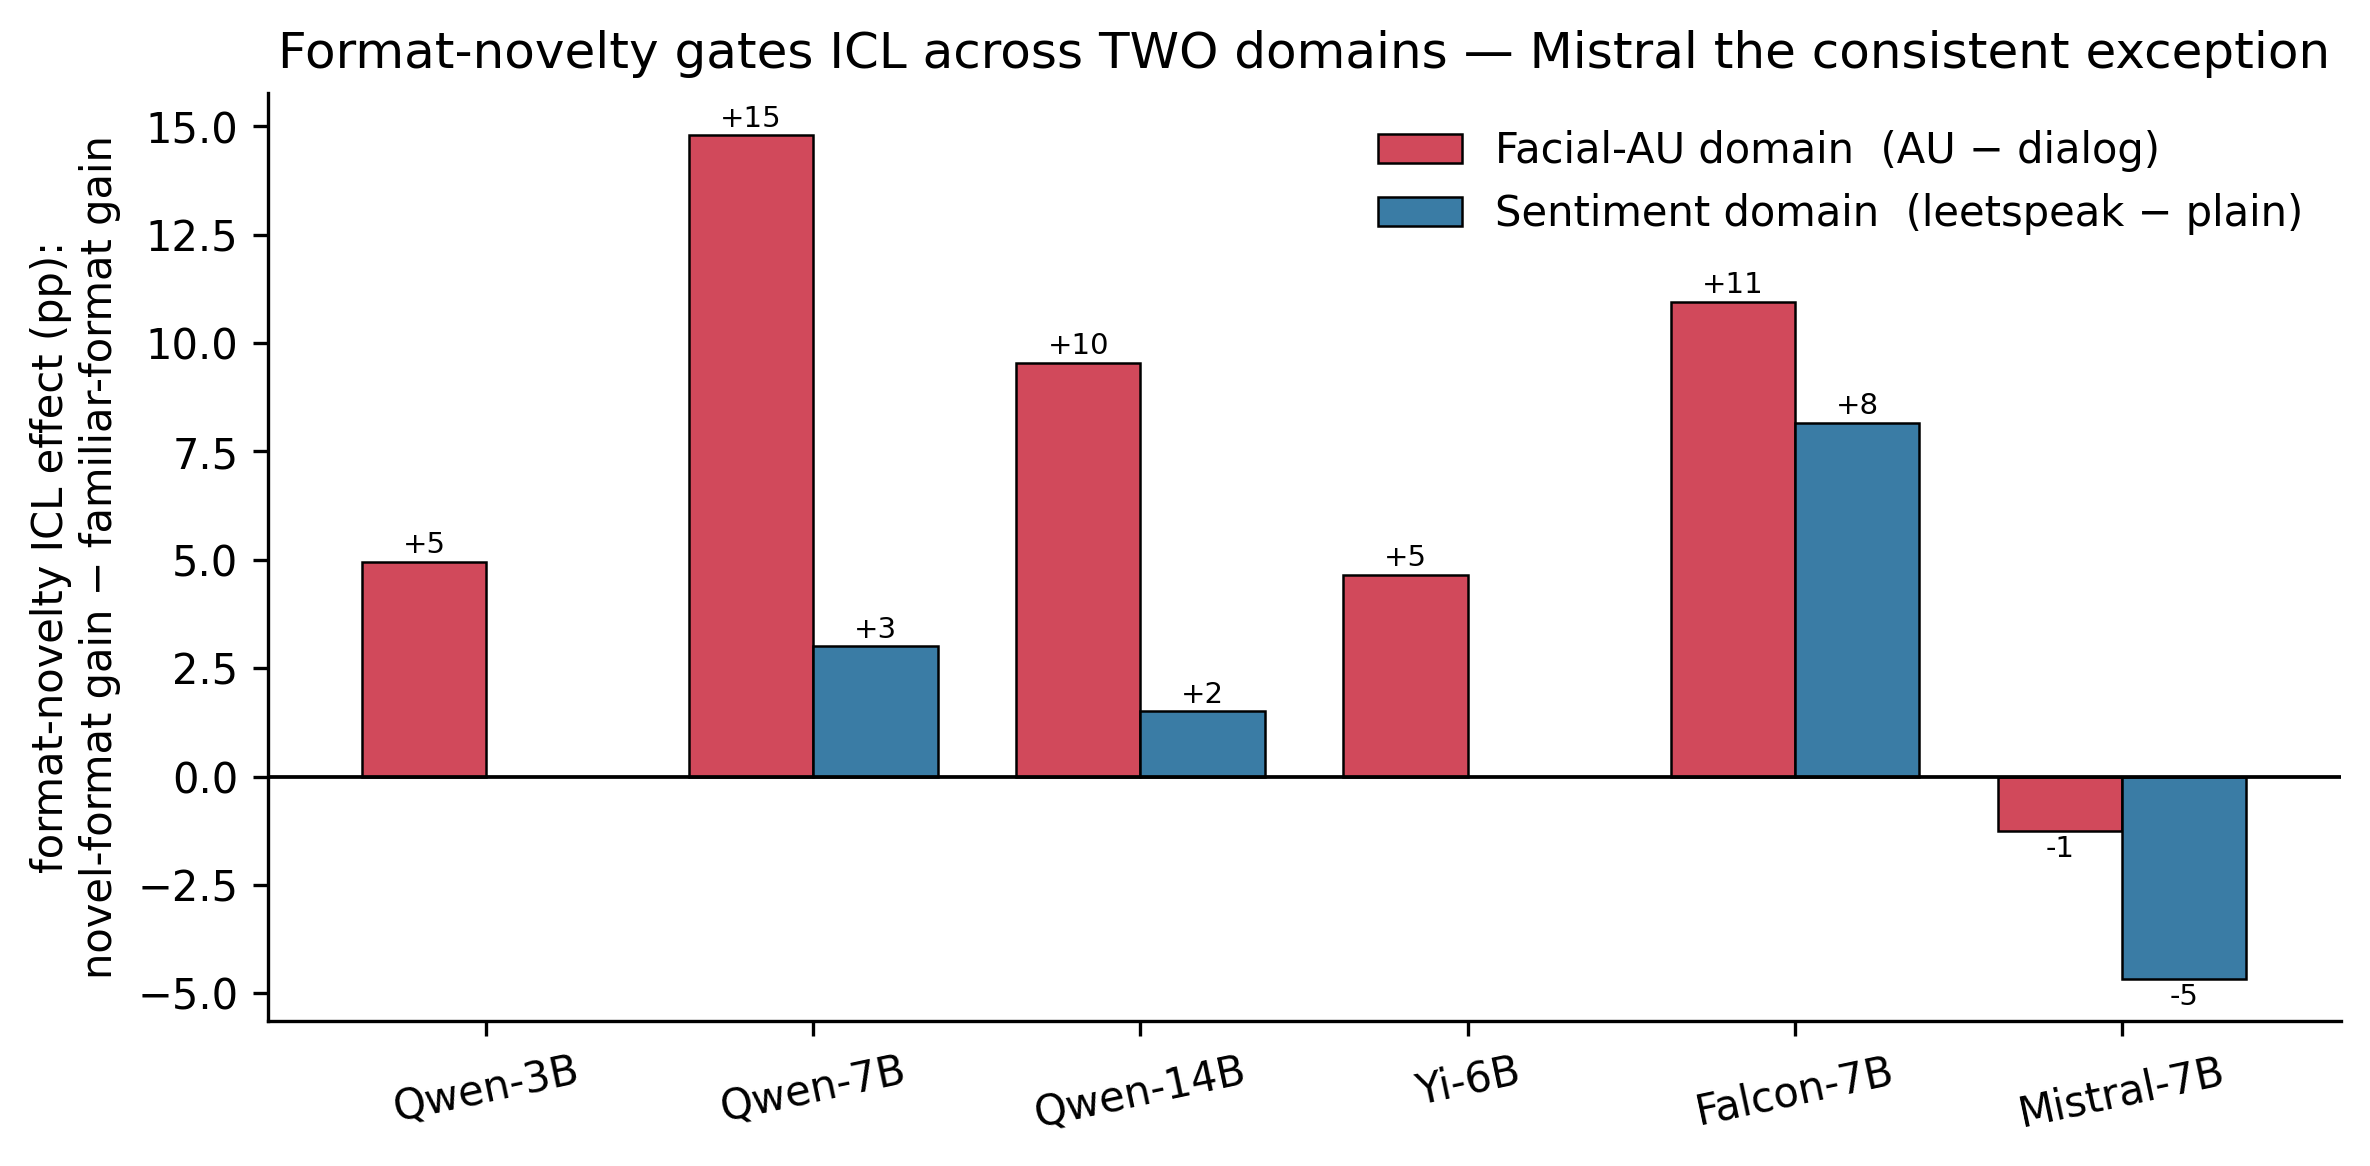
\includegraphics[width=\linewidth]{figures/figD_cross_domain.png}
\caption{Format-novelty ICL effect (novel$-$familiar gain) across two domains; Mistral is
the consistent exception.}\label{fig:cross}
\end{figure}

\subsection{Boundary condition: latent knowledge is necessary}\label{sec:boundary}
Format novelty alone is insufficient. Serializing a clinical tabular task (diabetes)
into an alien numeric format yields \emph{high} fertility ($5.8$, above AU) but
\emph{no} ICL gain (it hurts): the model has no latent ability for blood-value$\to$diagnosis,
so there is no task to recognize. This completes a $2\times2$: ICL gain is large only when
the task is latently known \emph{and} the format is novel.

\subsection{Negative controls and the exception}\label{sec:controls}
Beyond perplexity, the gain is not explained by \emph{headroom} (familiar IEMOCAP has
$+22$pp of LoRA headroom yet $\sim$0 ICL gain) nor by a single-vector
\emph{representation-compaction} account (no cross-model correlation, $\rho=0.31$, n.s.).
Mistral is a consistent null in \emph{both} domains; rather than noise, we read this as a
reproducible model-family property consistent with pretraining-corpus dependence
\cite{shin2022corpora,yadlowsky2023mixtures}.

\section{Discussion}
The picture is coherent: an LLM holds latent competence for many tasks, but an unfamiliar
input \emph{format} blocks cold zero-shot access to it. A few demonstrations---even with
wrong labels---re-establish the task frame (label space, output convention, what is being
asked), letting the model apply its priors. This is \emph{task recognition} in the sense
of \citet{pan2023tr}, here triggered by the \emph{format} rather than the task, and
quantifiable a priori by tokenizer fertility. It also predicts a failure mode at the
extreme: an encoding so alien that even recognition cannot be restored (cf.\ ciphered
reasoning), bounding a ``recoverable-novelty'' window.

\section{Limitations}
The second-domain (leetspeak) effect, while consistent in sign for 3/4 models, is smaller
than the AU effect ($+1.5$ to $+8.2$ vs.\ $+6.7$ to $+16.4$). One family (Mistral) does not
show the effect. Experiments use 4-bit models, $k{=}4$, $N{=}400$, and 5--7 seeds; the
emotion testbed is single-language. We characterize a phenomenon and its predictor rather
than provide a full mechanistic theory.

\section{Conclusion}
ICL is not a uniform lever: it pays off when demonstrations let an LLM \emph{recognize} a
latently-known task that an unfamiliar input format has hidden. Tokenizer fertility cheaply
predicts when this regime holds, and the effect replicates across model families and a
second domain. This sharpens practitioner guidance on when few-shot prompting is worth it.

\begin{thebibliography}{9}\small
\bibitem[Min et al.(2022)]{min2022rethinking} Min et al. Rethinking the Role of Demonstrations. EMNLP 2022.
\bibitem[Pan et al.(2023)]{pan2023tr} Pan et al. Disentangling Task Recognition and Task Learning. ACL Findings 2023.
\bibitem[Fu et al.(2024)]{fu2024isobench} Fu et al. IsoBench. COLM 2024.
\bibitem[Hegselmann et al.(2023)]{hegselmann2023tabllm} Hegselmann et al. TabLLM. AISTATS 2023.
\bibitem[Shin et al.(2022)]{shin2022corpora} Shin et al. Effect of Pretraining Corpora on ICL. NAACL 2022.
\bibitem[Yadlowsky et al.(2023)]{yadlowsky2023mixtures} Yadlowsky et al. Pretraining Data Mixtures. 2023.
\bibitem[Razeghi et al.(2022)]{razeghi2022impact} Razeghi et al. Impact of Pretraining Term Frequencies. EMNLP Findings 2022.
\end{thebibliography}
\end{document}
